\documentclass[11pt,a4paper]{article}
\usepackage{fontspec}
\setmainfont{DejaVu Serif}
\setmonofont{DejaVu Sans Mono}
\usepackage{amsmath,amssymb,bm}
\usepackage{booktabs,array}
\usepackage[xetex]{graphicx}
\usepackage{xcolor,hyperref,listings}
\usepackage[margin=24mm]{geometry}
\hypersetup{colorlinks=true,linkcolor=blue,urlcolor=blue}
\lstset{language=C,basicstyle=\ttfamily\small,
 keywordstyle=\color{blue!65!black},commentstyle=\color{green!40!black},
 stringstyle=\color{red!55!black},numbers=left,numberstyle=\tiny\color{gray},
 frame=single,breaklines=true,columns=fullflexible,keepspaces=true}

\title{Implementation of a Two-Electrode Fixed Potential-Difference Method\\
in OpenMX 3.9.9}
\author{}
\date{July 2026}

\begin{document}
\maketitle
\tableofcontents

\section{Purpose and scope}

This extension adds a minimal fixed electrode potential-difference capability
to OpenMX 3.9.9. Two sets of atoms define left and right electrodes. The fixed
input $V_c$ applies $+V_c/2$ to the left group and $-V_c/2$ to the right group;
the constraint-potential difference is therefore $V_c$. The transferred
charge is determined self-consistently.

The implementation covers input parsing, electrode assignment, Mulliken
population sums, an unconstrained reference state, the constraint
Hamiltonian, fixed-$V_c$ convergence tests, and output. It does not implement
target-charge feedback, constraint forces, constraint-energy
corrections, restart persistence, multiple constraints, or NEGF coupling.

\section{Definitions and derivation}

\subsection{Mulliken populations and transferred charge}

Let $P_{\mu\nu}$ and
$S_{\mu\nu}=\langle\phi_\mu|\phi_\nu\rangle$ denote the density and overlap
matrices in a non-orthogonal atomic-orbital basis. The Mulliken electron
population assigned to atom $A$ is
\begin{equation}
 N_A=\sum_{\mu\in A}\sum_\nu P_{\mu\nu}S_{\nu\mu}.
\end{equation}
The electrode populations are
\begin{equation}
 N_L=\sum_{A\in L}N_A,\qquad N_R=\sum_{A\in R}N_A.
\end{equation}
An ordinary $V_c=0$ calculation is converged first. Its populations
$N_L^0,N_R^0$ define
\begin{equation}
 \Delta N_L=N_L-N_L^0,\qquad \Delta N_R=N_R-N_R^0.
\end{equation}
Positive transfer is defined as electron loss from the left and gain by the
right electrode:
\begin{equation}
 Q=\frac{-\Delta N_L+\Delta N_R}{2}.
 \label{eq:q}
\end{equation}
For a charge-conserving two-electrode system,
$\Delta N_L+\Delta N_R=0$ and Eq.~\eqref{eq:q} reduces to
$Q=-\Delta N_L=\Delta N_R$. The factor $1/2$ prevents double counting.

\subsection{Constrained functional}

Introduce an electrode weight
\begin{equation}
 w(\bm r)=\begin{cases}
 +1,&\bm r\in L,\\-1,&\bm r\in R,\\0,&\text{otherwise}.
 \end{cases}
\end{equation}
A functional containing the fixed external electrode potential is
\begin{equation}
 W[n;V_c]=E_{\rm DFT}[n]+\frac{V_c}{2}\int w(\bm r)n(\bm r)d\bm r.
\end{equation}
Variation with respect to $n$ adds
\begin{equation}
 V_{\rm con}(\bm r)=\frac{V_c}{2}w(\bm r)
\end{equation}
to the Kohn--Sham potential. $V_c$ is fixed input rather than a varied
Lagrange multiplier. The induced transfer is measured using the Mulliken
atomic partition of Eq.~\eqref{eq:q}.

A positive $V_c$ raises electron levels on the left and lowers them on the
right. Thus positive $V_c$ drives the positive charge-transfer convention.

\subsection{Euler--Lagrange equation and ensemble}

The semicolon in $W[n;V_c]$ is important: $V_c$ is prescribed and variation
is performed only with respect to the density, subject to the ordinary total
electron-number normalization. Introducing the chemical potential $\mu$ for
that normalization gives
\begin{equation}
 \frac{\delta}{\delta n(\bm r)}
 \left\{E_{\rm DFT}[n]+\frac{V_c}{2}\int w n\,d\bm r
 -\mu\left(\int n\,d\bm r-N_e\right)\right\}=0,
\end{equation}
or
\begin{equation}
 \frac{\delta E_{\rm DFT}}{\delta n(\bm r)}+\frac{V_c}{2}w(\bm r)=\mu.
 \label{eq:euler-fixed-vc}
\end{equation}
The self-consistent density is therefore stationary for a fixed external
electrode field. This is distinct from target-charge cDFT, where $V_c$ is
also varied and $\partial W/\partial V_c=0$ enforces a specified population.
No such second stationarity condition or target population exists here.

For conserved total charge, Eq.~\eqref{eq:q} implies
\begin{equation}
 N_L-N_R={\rm constant}-2Q.
\end{equation}
The field-dependent part of the reduced functional is consequently
\begin{equation}
 \mathcal F(Q;V_c)=E_{\rm DFT}(Q)-V_cQ+{\rm constant}.
\end{equation}
Stationarity with respect to the induced transfer gives
\begin{equation}
 \frac{dE_{\rm DFT}}{dQ}=V_c.
 \label{eq:conjugate-vc}
\end{equation}
Thus $V_c$ is the field conjugate to $Q$ and the imposed constraint-potential
difference. It is not the self-consistent Hartree voltage
$\Delta\phi_H$, which must be read independently from the Hartree grid.

Equation~\eqref{eq:euler-fixed-vc} establishes density stationarity for the
implemented one-electron problem. A stronger statement about OpenMX total
energies and forces would require adding $\mathrm{Tr}[P H^{\rm con}]$ to the
reported energy with consistent double-counting treatment, and differentiating
the overlap-dependent matrix with respect to atomic positions. Those energy,
force, and stress terms are not implemented. Consequently fixed-geometry
densities, charges, and potentials are supported, but constrained energy
comparisons and geometry optimization are not variationally supported.

\section{Constraint matrix in a non-orthogonal basis}

Suppose the local constraint takes atom-centered values $V_A$. The exact
two-center matrix element is
\begin{equation}
 \langle\phi_{A\mu}|V_{\rm con}|\phi_{B\nu}\rangle
 =\int\phi_{A\mu}^*(\bm r)V_{\rm con}(\bm r)
 \phi_{B\nu}(\bm r)d\bm r.
\end{equation}
Approximating the potential in the overlap region by the symmetric endpoint
average yields
\begin{align}
 H^{\rm con}_{A\mu,B\nu}
 &\simeq\frac{V_A+V_B}{2}
 \int\phi_{A\mu}^*(\bm r)\phi_{B\nu}(\bm r)d\bm r\\
 &=\frac{V_A+V_B}{2}S_{A\mu,B\nu}.
 \label{eq:hcon}
\end{align}
This expression is Hermitian and reduces to a diagonal on-site shift in an
orthogonal basis. The atom value is
\begin{equation}
 V_A=\begin{cases}+V_c/2,&g_A=1,\\-V_c/2,&g_A=2,\\0,&g_A=0.
 \end{cases}
\end{equation}
Input values are in eV and are divided by 27.2113845 before addition to the
Hartree-unit OpenMX Hamiltonian.

The scalar potential is added to both spin-diagonal blocks in a
non-collinear calculation and not to spin-off-diagonal blocks. It is added
before orbital contraction so that the existing contraction path transforms
the complete Hamiltonian consistently.

\section{Fixed potential-difference control}

The robust sweep mode is enabled by
\begin{lstlisting}[language={}]
Potential.Constraint.Vc 0.24
\end{lstlisting}
The code converges the $V_c=0$ reference, switches on the specified fixed
potential, waits at least three constrained iterations, and then terminates
when the electronic-energy criterion is met. The finite polarization itself
can leave a nonzero density metric, so that metric is not used as the sole
fixed-$V_c$ termination condition.

Independent calculations provide $Q(V_c)$ and the Hartree response. There is
no target-charge, proportional-feedback, or variable-$V_c$ input mode.

\section{Hartree sign and capacitance}

OpenMX \texttt{dVHart} is an electron potential energy entering the
one-electron Hamiltonian. Since the electron charge is $-e$, the physical
electrostatic potential is
\begin{equation}
 \phi(\bm r)=-\frac{V_H(\bm r)}{e}.
 \label{eq:sign}
\end{equation}
Thus
\begin{equation}
 \Delta\phi_{R-L}=-\frac{V_H(R)-V_H(L)}{e}.
\end{equation}
Correcting this sign reverses voltage polarity but does not alter the
positive capacitance magnitude
\begin{equation}
 C_{\rm total}=\frac{|Q|e}{|\Delta\phi|},\qquad
 \frac{C_{\rm total}}{A}=\frac{|Q|e}{|\Delta\phi|A}.
\end{equation}
The analysis program plane-averages the Hartree cube,
\begin{equation}
 \overline V_H(x)=\frac{1}{A}\int_A V_H(x,y,z)dy\,dz,
\end{equation}
and interpolates it at the two electrode coordinates.

The fixed external constraint difference is not automatically identical to
the Hartree voltage. If an electrochemical voltage is required, the contribution
conjugate to charge transfer must be defined thermodynamically; identifying
it with $V_c$, or combining it with the Hartree drop, requires an explicit
and consistent sign convention.

\section{Input syntax}

\begin{lstlisting}[language={}]
Potential.ConstraintDFT        on
Potential.Constraint.Vc        0.24
Potential.Constraint.Output    on

<Potential.Constraint
1  1
2  1
3  2
4  2
Potential.Constraint>
\end{lstlisting}
Group 0 is unconstrained, group 1 is the left electrode, and group 2 is the
right electrode. Omitted atoms remain in group 0. The parser validates atom
indices, group values, and the existence of both electrode groups.

\section{Detailed source modifications}

\subsection{\texttt{openmx\_common.h}}
The header defines enable/output flags, the atom-group array, reference-state
flags and iteration, fixed $V_c$, current and reference populations,
transferred charge, and the function prototypes.

\subsection{\texttt{Input\_std.c}}
New scalar keywords are read with backward-compatible defaults. After the
normal atom arrays are allocated, \texttt{PotentialConstraintGroup} is
allocated and initialized to zero. The independent block is parsed after
the standard coordinates. NEGF is rejected because it is outside the MVP.

\subsection{\texttt{Set\_Hamiltonian.c}}
After construction of the ordinary uncontracted Hamiltonian, the code
evaluates the atom values $V_A,V_B$ and applies Eq.~\eqref{eq:hcon}:
\begin{lstlisting}
vA = group[A]==1 ? +Vc/2 : group[A]==2 ? -Vc/2 : 0.0;
vB = group[B]==1 ? +Vc/2 : group[B]==2 ? -Vc/2 : 0.0;
dv = 0.5*(vA + vB)/eV2Hartree;
H[spin][A][B][mu][nu] += dv*OLP[0][A][B][mu][nu];
\end{lstlisting}
The constraint is inactive until the reference state has converged.

\subsection{\texttt{Potential\_Constraint.c}}
This new file contains population aggregation, initialization, reference
capture, fixed-$V_c$ reporting, and final reporting. OpenMX has already gathered
per-atom Mulliken populations to the host after
\texttt{Mulliken\_Charge()}; the host sums the groups and broadcasts the
two totals to all ranks.

\subsection{\texttt{DFT.c}}
The DFT driver initializes the state, evaluates the populations after every
Mulliken analysis, and captures the first converged unconstrained reference.
The maximum SCF count is doubled to accommodate reference and constrained
stages. The fixed-$V_c$ calculation uses its dedicated convergence rule and minimum
post-reference iteration count. A final summary is emitted after the final
Mulliken analysis.

\subsection{\texttt{makefile} and analysis programs}
\texttt{Potential\_Constraint.o} is added to the OpenMX object list. The minimal
distribution patch does not alter compiler or library paths.
\texttt{capacitance\_from\_vhart.py} performs cube averaging, sign conversion,
and unit conversion. \texttt{plot\_v\_ct.py} collects a sweep into CSV and
creates Q--V and V--$C_{\rm total}/A$ figures.

\section{Positive and negative sweep for $d=10.05$~\AA}

Fixed $V_c$ calculations were performed with ESM on1 for both polarities.
Apart from a constant, the constraint energy is
\begin{equation}
 E_{\rm con}=\frac{V_c}{2}(N_L-N_R)=-V_cQ.
\end{equation}
Stationarity at fixed transferred charge gives
\begin{equation}
 \frac{\partial E_{\rm DFT}}{\partial Q}=V_c.
\end{equation}
The voltage conjugate to charge transfer is therefore evaluated as
$V_{\rm total}=V_c$, and
\begin{equation}
 \frac{C_{\rm total}}{A}=\frac{|Q|e}{|V_c|A}.
\end{equation}
This is not an instruction to add $V_c$ to the Hartree voltage.

The Hartree geometric capacitance and an effective quantum/electronic
capacitance are
\begin{align}
 \frac{C_{\rm geom}}{A}&=\frac{|Q|e}{|\Delta\phi_H|A},\\
 \frac{1}{C_Q}&=\frac{1}{C_{\rm total}}-\frac{1}{C_{\rm geom}}.
\end{align}

\begin{table}[htbp]
\centering
\caption{Capacitance components in $\mu$F/cm$^2$.}
\begin{tabular}{rrrrr}
\toprule
$V_c$ (V)&$Q$ (e)&$C_{\rm geom}/A$&$C_{\rm total}/A$&$C_Q/A$\\
\midrule
-0.64&-0.00126618&1.07236&0.59993&1.36177\\
-0.48&-0.00087786&1.07237&0.55459&1.14860\\
-0.32&-0.00053004&1.07249&0.50228&0.94472\\
-0.16&-0.00023935&1.07231&0.45363&0.78624\\
 0.16& 0.00023935&1.07231&0.45363&0.78624\\
 0.32& 0.00053004&1.07249&0.50228&0.94472\\
 0.48& 0.00087786&1.07237&0.55459&1.14860\\
 0.64& 0.00126618&1.07237&0.59993&1.36176\\
\bottomrule
\end{tabular}
\end{table}

\begin{figure}[htbp]
\centering
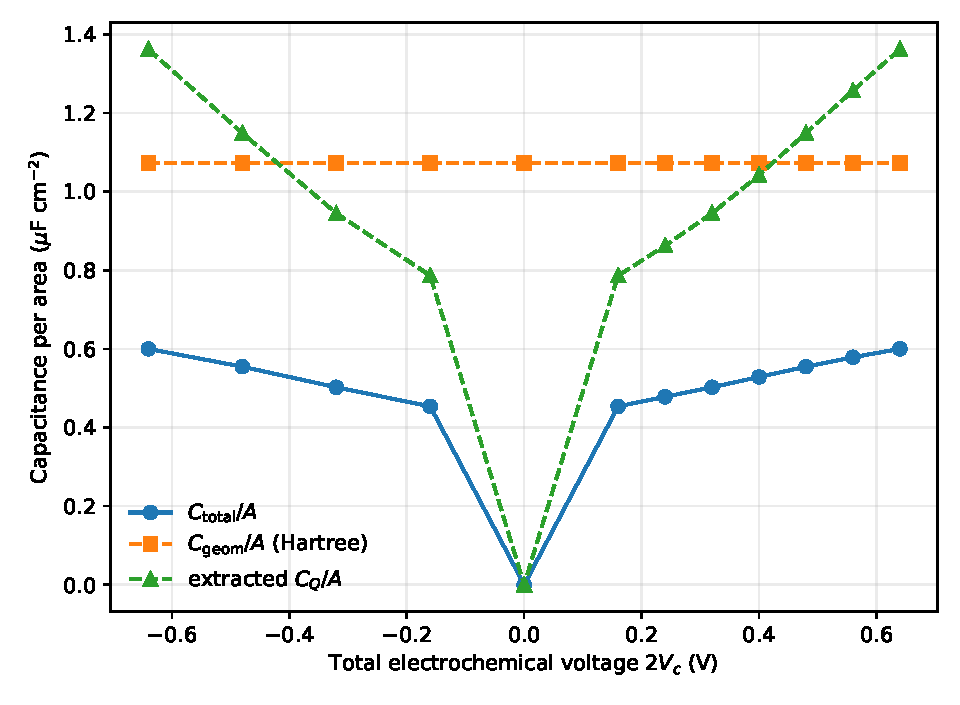
\includegraphics[bb=0 0 461 338,width=0.82\linewidth]{source/paper_reproduction/graphene_d10.05_capacitance_components.pdf}
\caption{Total, Hartree geometric, and series-extracted quantum/electronic
capacitances for $d=10.05$~\AA. The negative branch consists of independent
A/B-reversed calculations, not mirrored positive data.}
\end{figure}

$C_{\rm geom}/A$ remains constant at approximately
$1.0724~\mu$F/cm$^2$, as expected from the linear Poisson response at fixed
geometry. $C_{\rm total}/A$ increases with $|V_{\rm total}|$ and forms a
symmetric V-shaped curve. The extracted $C_Q$ is an effective non-Hartree
electronic contribution contained in the fixed-potential energy response, rather than
a direct density-of-states calculation. The plotted origin follows the
paper-style convention $C_{\rm total}(0)=0$; a rigorous zero-bias
differential capacitance requires closer-to-zero points and $dQ/dV$.

For a DOS-based comparison the two electrodes must be treated separately.
Let $D_L(E)$ and $D_R(E)$ be layer-projected DOSs per cell in states/eV.
Then
\begin{align}
 \frac{C_{Q,L}^{\rm DOS}}{A}&=\frac{e}{A}\int D_L(E)
 \left[-\frac{\partial f(E-\mu_L,T)}{\partial E}\right]dE,\\
 \frac{C_{Q,R}^{\rm DOS}}{A}&=\frac{e}{A}\int D_R(E)
 \left[-\frac{\partial f(E-\mu_R,T)}{\partial E}\right]dE,\\
 \frac{1}{C_{Q,\rm transfer}^{\rm DOS}}&=
 \frac{1}{C_{Q,L}^{\rm DOS}}+\frac{1}{C_{Q,R}^{\rm DOS}},\\
 C_{Q,\rm transfer}^{\rm DOS}&=
 \frac{C_{Q,L}^{\rm DOS}C_{Q,R}^{\rm DOS}}
 {C_{Q,L}^{\rm DOS}+C_{Q,R}^{\rm DOS}}.
\end{align}
The $e/A$ prefactor applies when energy and DOS use eV; the equivalent SI
formula in joules has prefactor $e^2/A$.  For equivalent layers at zero bias,
$C_{Q,\rm transfer}^{\rm DOS}=C_{Q,\rm layer}^{\rm DOS}/2$. Since then
$D_{\rm bilayer}=2D_{\rm layer}$,
\begin{equation}
 \frac{C_{Q,\rm transfer}^{\rm DOS}}{A}=\frac{e}{4A}\int
 D_{\rm bilayer}(E)\left[-\frac{\partial f(E-\mu,T)}{\partial E}\right]dE.
\end{equation}
Using the total bilayer DOS as one electrode would overestimate the transfer
capacitance by a factor of four. At short distance the layer DOS is
projection-dependent because of hybridization.

We evaluated this comparison at 300~K using zero-bias OpenMX layer PDOSs on
a $1\times300\times300$ k grid and 0.005~eV Gaussian broadening.  At every
fixed-$V_c$ point, the non-Hartree voltage
$V_Q=V_c-\Delta\phi_H$ was mapped symmetrically to
$\mu_L=+V_Q/2$ and $\mu_R=-V_Q/2$.  The resulting layer capacitances were
then combined in series.
\begin{figure}[htbp]
\centering
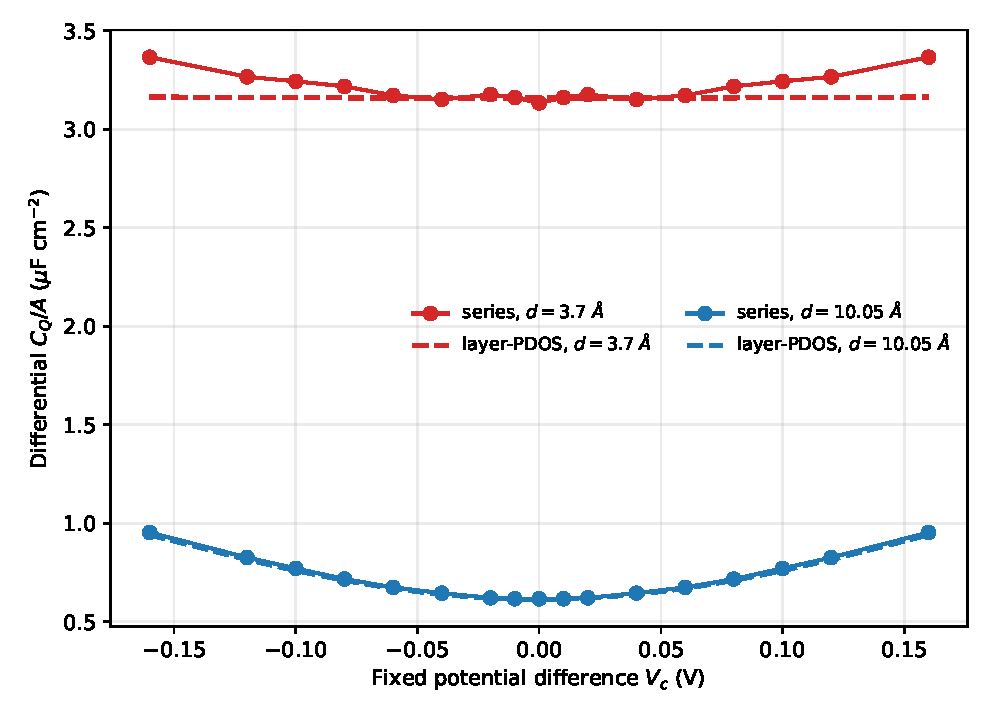
\includegraphics[bb=0 0 475 346,width=0.84\linewidth]{source/paper_reproduction/graphene_cq_dos_vs_series_300k.pdf}
\caption{Comparison at 300~K between differential $C_Q$ extracted from the
fixed-$V_c$ series relation (solid) and the layer-PDOS transfer capacitance
(dashed).}
\end{figure}
At $V_c=0$, the series and DOS results are respectively 3.134 and
$3.159~\mu$F/cm$^2$ for $d=3.70$~\AA, and 0.616 and
$0.613~\mu$F/cm$^2$ for $d=10.05$~\AA.  At 0.16~V the corresponding pairs
are 3.366 versus 3.164 and 0.953 versus 0.941.  Thus the long-distance DOS
calculation reproduces both the thermally rounded Dirac minimum and its rise
with voltage.  At short distance both methods instead give a finite, nearly
flat response near $3.1~\mu$F/cm$^2$, consistent with strong hybridization.
Finite-voltage differences include rigid-band, self-consistent band-change,
and layer-projection effects.

\section{Comparison with the paper and experimental meaning}

Table~\ref{tab:papercomparison} compares the results for $d=10.05$~\AA{} at
a voltage magnitude near 0.6~V. The charge inferred from the published
capacitance uses the same primitive-cell area, $5.28353$~\AA$^2$.

\begin{table}[htbp]
\centering
\caption{Comparison with the published result. Capacitances are in
$\mu$F/cm$^2$.}
\label{tab:papercomparison}
\small
\begin{tabular}{lrr}
\toprule
Case & $C/A$ & $Q$ (e/cell)\\
\midrule
Sohib et al. & $\sim2.25$ & $\sim0.00445$ (inferred)\\
ESM-on4 reproduction at 0.584 V & 2.7166 & 0.005233962\\
ESM-on1 fixed-$V_c$ near 0.6 V & $\sim0.59$ & $\sim0.00117$\\
Hartree geometric value & $\sim1.0724$ & $\sim0.00117$\\
\bottomrule
\end{tabular}
\end{table}

The fixed-$V_c$ total capacitance has the same $1~\mu$F/cm$^2$ order of
magnitude and reproduces the symmetric V-shaped trend, but it is only about
26\% of the quoted value and is not quantitative agreement. The ESM-on4
reproduction is much closer to the paper. The principal distinction is the
boundary condition and voltage definition. ESM on4 with
\texttt{ESM.potential.diff} imposes an external field across the cell, whereas
ESM on1 with the local $+V_c/2,-V_c/2$ potential drives charge transfer directly
while removing the nonperiodic image interaction. Furthermore, $V_c$ is the
variable conjugate to $Q$ in the fixed-potential functional; it is neither the Hartree
potential difference nor a correction to be added to it. Stacking, ESM
boundary positions, unreleased author-specific ESM changes, charge
partitioning, and the distinction between secant and differential
capacitance can add further differences. Carbon SOC is unlikely to account
for the approximately fourfold charge discrepancy.

The correspondence to experiment depends on the measurement. The
Hartree-only $C_{\rm geom}$ is an electrostatic geometric capacitance. A
two-terminal voltage normally measures an electrochemical-potential
difference, so its small-signal capacitance contains geometric and quantum
contributions in series:
\begin{equation}
 C_{\rm meas}=\frac{dQ}{dV_{\rm electrochemical}},\qquad
 \frac{1}{C_{\rm meas}}=\frac{1}{C_{\rm geom}}+\frac{1}{C_Q}.
\end{equation}
In this sense, the ESM-on1 constrained calculation is conceptually closer to
an image-free two-terminal capacitor, whereas ESM on4 is the appropriate
comparison for the paper's externally driven protocol. A direct small-signal
comparison must use $dQ/d(V_c)$ rather than the finite-bias secant
$Q/(V_c)$ and must test the Mulliken group dependence. Neither the present
$C_{\rm total}$ nor the paper's Hartree-based ratio should therefore be
identified with an experimental terminal capacitance without these
qualifications.

\section{Stock-OpenMX reanalysis of the Sohib protocol}

We performed a stock OpenMX 3.9.9 ESM-on4 sweep at 300~K for six distances
$d=3.70$, 5.82, 7.93, 10.05, 12.17, and 14.29~\AA{} and for
$V_{\rm ESM}=0.4$, 0.8, 1.2, 1.6, 2.0, and 2.6~V, using the paper's
$1\times100\times100$ SCF k grid. Following Sohib et al., the operational
total capacitance is
\begin{equation}
 \frac{C_{\rm total}^{\rm Sohib}}{A}
 =\frac{|Q|e}{A|\Delta V_H^{\rm raw}|},
\end{equation}
where $\Delta V_H^{\rm raw}$ is the layer-to-layer difference read directly
from the OpenMX \texttt{.vhart} cube. The layer-PDOS capacitances at 300~K
are
\begin{align}
 \frac{C_{Q,i}^{\rm DOS}}{A}&=\frac{e}{A}\int D_i(E)
 \left[-\frac{\partial f(E-\mu_i,T)}{\partial E}\right]dE,\\
 \mu_L&=+\Delta V_H^{\rm raw}/2,\qquad
 \mu_R=-\Delta V_H^{\rm raw}/2,\\
 \frac{1}{C_{Q,\rm transfer}^{\rm DOS}}&=
 \frac{1}{C_{Q,L}^{\rm DOS}}+\frac{1}{C_{Q,R}^{\rm DOS}}.
\end{align}
The remaining series component is defined by
\begin{equation}
 \frac{1}{C_{\rm geom}^{\rm eff}}=
 \frac{1}{C_{\rm total}^{\rm Sohib}}-
 \frac{1}{C_{Q,\rm transfer}^{\rm DOS}}.
\end{equation}

\begin{figure}[htbp]
\centering
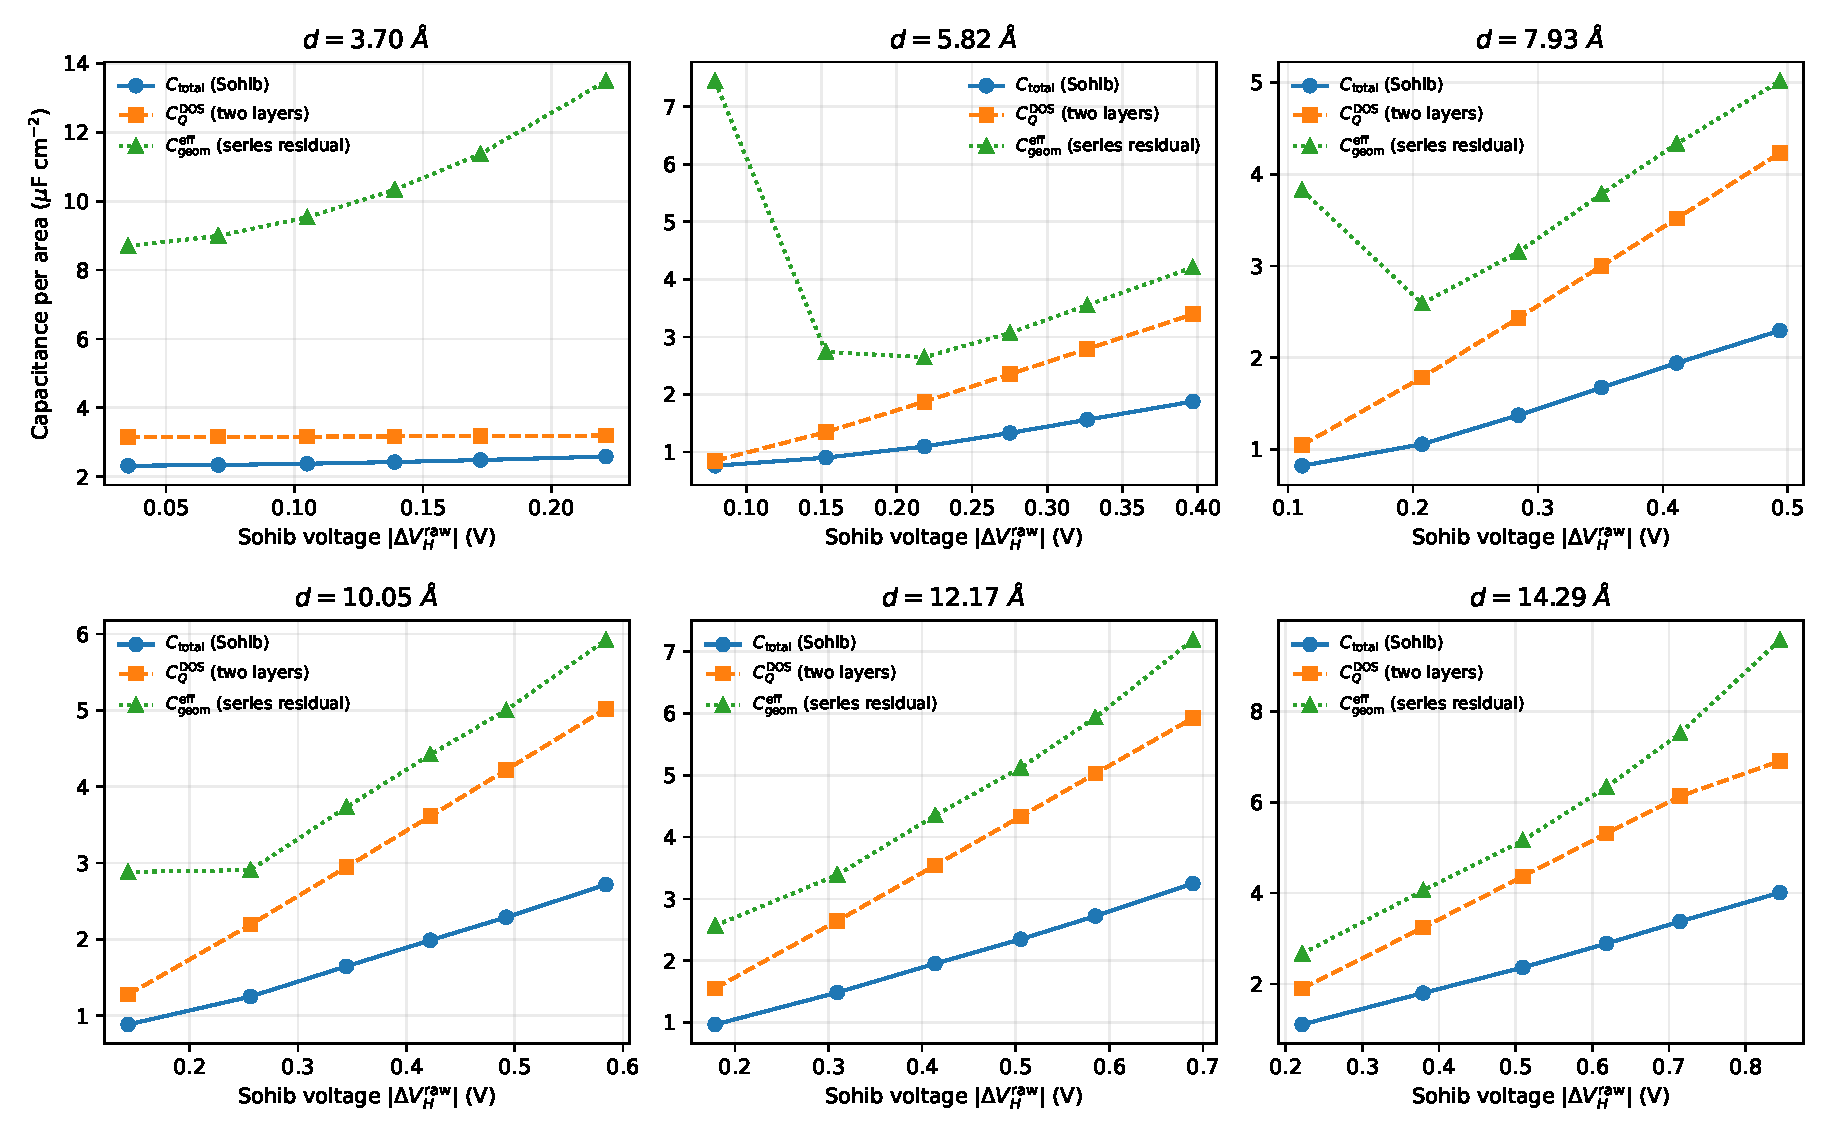
\includegraphics[bb=0 0 734 302,width=0.96\linewidth]{source/paper_reproduction/sohib_stock_openmx_capacitance_components.pdf}
\caption{Stock-OpenMX ESM-on4 reanalysis. The total follows the raw-Hartree
definition of Sohib et al.; $C_Q$ is obtained from the two layer DOSs, and
$C_{\rm geom}^{\rm eff}$ is the algebraic series residual.}
\end{figure}

At $V_{\rm ESM}=2.6$~V, the triples
$(C_{\rm total}^{\rm Sohib},C_{Q,\rm transfer}^{\rm DOS},C_{\rm geom}^{\rm eff})/A$
for increasing $d$ are $(2.584,3.197,13.484)$, $(1.879,3.395,4.209)$,
$(2.295,4.232,5.014)$, $(2.717,5.019,5.922)$, $(3.247,5.923,7.188)$,
and $(4.011,6.906,9.571)$, in $\mu$F/cm$^2$. These residual values are not
classical vacuum geometric capacitances. Stock OpenMX adds the external ESM-on4 ramp directly to
\texttt{dVHart\_Grid\_B}, so the raw cube contains both external and induced
terms. After subtracting the analytic external ramp, the induced-Hartree
diagnostic gives 2.201, 2.072, 2.109, 2.197, 2.507, and 3.347~$\mu$F/cm$^2$.
The signed external difference is $\Delta V_{\rm ext}^{R-L}=-V_{\rm ESM}d/L$,
as follows from the $-0.5V_{\rm ESM}(z-z_1)/z_1$ term in
\texttt{Poisson\_ESM.c};
$\epsilon_0/d$ gives 2.393, 1.521, 1.116, 0.881, 0.728, and 0.620~$\mu$F/cm$^2$.

\begin{figure}[htbp]
\centering
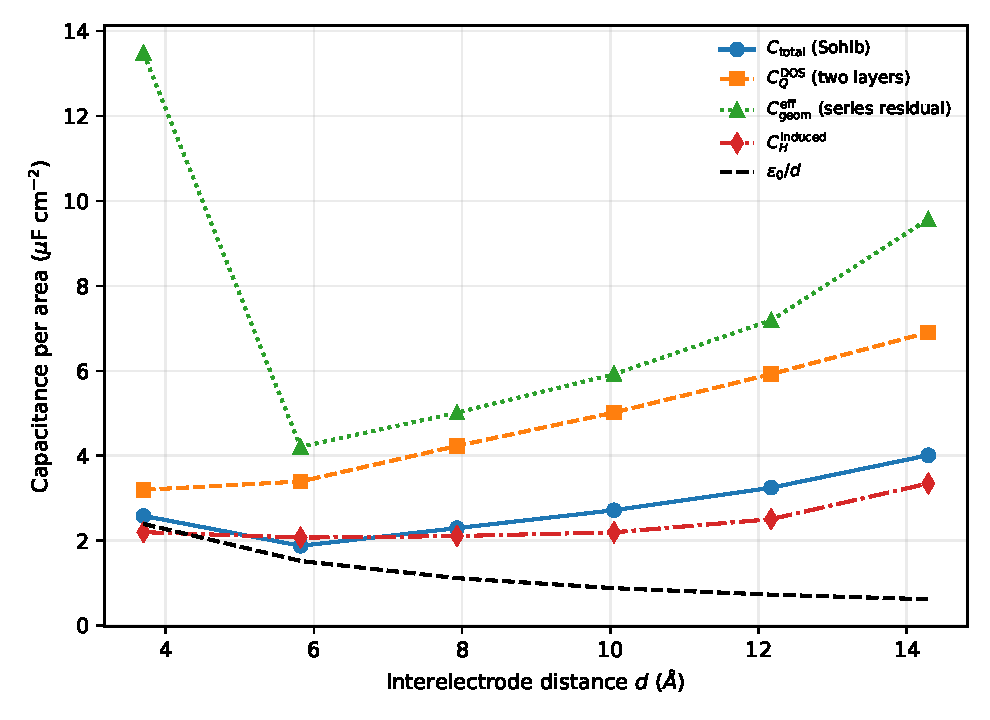
\includegraphics[width=0.78\linewidth]{source/paper_reproduction/sohib_stock_openmx_distance_dependence.pdf}
\caption{Distance dependence at $V_{\rm ESM}=2.6$~V.}
\end{figure}

This diagnostic is not a pure geometric capacitance across the series:
short-distance overlap and charge partitioning matter, while at
$d=14.29$~\AA{} the sheet--ESM clearance is only 2.855~\AA{} in the 20~\AA{}
cell and boundary/contact effects contaminate the endpoint. Thus the agreement
near 10.05~\AA{} is not a general validation, and $C_{\rm geom}^{\rm eff}$ is
more accurately an effective other/series capacitance.

\subsection{ESM-boundary convergence}

We repeated the three largest distances in a 30~\AA{} cell. Because fixed
$V_{\rm ESM}$ would reduce the applied field when increasing the cell, the
30~\AA{} values were scaled by $30/20=1.5$; hence 2.6~V in the 20~\AA{} cell
is compared with 3.9~V in the 30~\AA{} cell. This keeps both the external
field and $V_{\rm ESM}d/L$ fixed.
\begin{center}
\begin{tabular}{rrrrrr}
\toprule
$d$ (\AA)&edge$_{20}$&edge$_{30}$&$C_{H,20}^{\rm ind}/A$&$C_{H,30}^{\rm ind}/A$&$\epsilon_0/d$\\
\midrule
10.05&4.975&9.975&2.197&1.420&0.881\\
12.17&3.915&8.915&2.507&1.357&0.728\\
14.29&2.855&7.855&3.347&1.346&0.620\\
\bottomrule
\end{tabular}
\end{center}
Capacitances are in $\mu$F/cm$^2$. Increasing the clearance reduces the
14.29~\AA{} value from 3.347 to 1.346, confirming strong ESM-boundary
contamination in the 20~\AA{} cell. The nearly flat 30~\AA{} trend remains
about 1.5--2.2 times $\epsilon_0/d$, so this Hartree diagnostic is not the
ideal parallel-plate capacitance.
\begin{figure}[htbp]
\centering
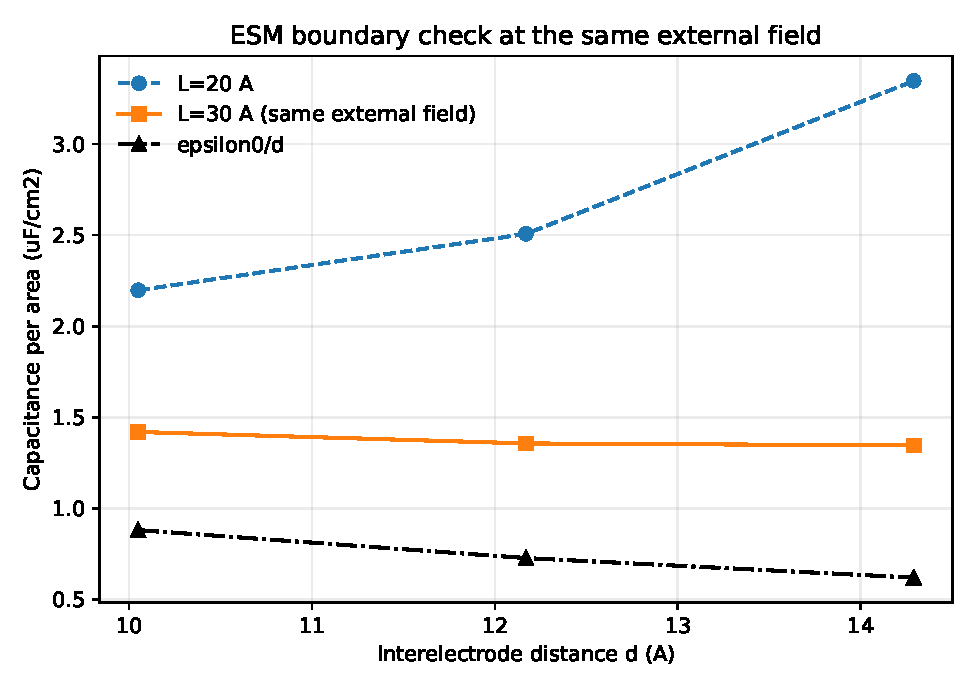
\includegraphics[width=0.76\linewidth]{source/paper_reproduction/sohib_L30_boundary_check.pdf}
\caption{ESM-boundary convergence at the same external field.}
\end{figure}

\section{Two distances: analogues of Fig.~4(b) and 4(c)}

The same ESM-on1 fixed-$V_c$ sweep was performed for $d=3.70$ and
10.05~\AA. At $|V_c|=0.6$~V, linear interpolation gives
\begin{center}
\begin{tabular}{rrrrr}
\toprule
$d$ (\AA)&$Q$ (e/cell)&$C_{\rm total}/A$&$C_{\rm geom}/A$&$C_Q/A$\\
\midrule
3.70&0.00469&2.37&5.98&3.92\\
10.05&0.00117&0.589&1.072&1.31\\
\bottomrule
\end{tabular}
\end{center}
Capacitances are in $\mu$F/cm$^2$. The paper reports approximately 3.4 and
2.25, respectively, so the present totals are about 70\% and 26\% of those
values. The short-distance $C_{\rm geom}$ decreases mildly from 6.22 to 5.96
over the sweep, indicating interlayer-overlap effects; it remains nearly
constant at 1.0724 for 10.05~\AA.

\begin{figure}[htbp]
\centering
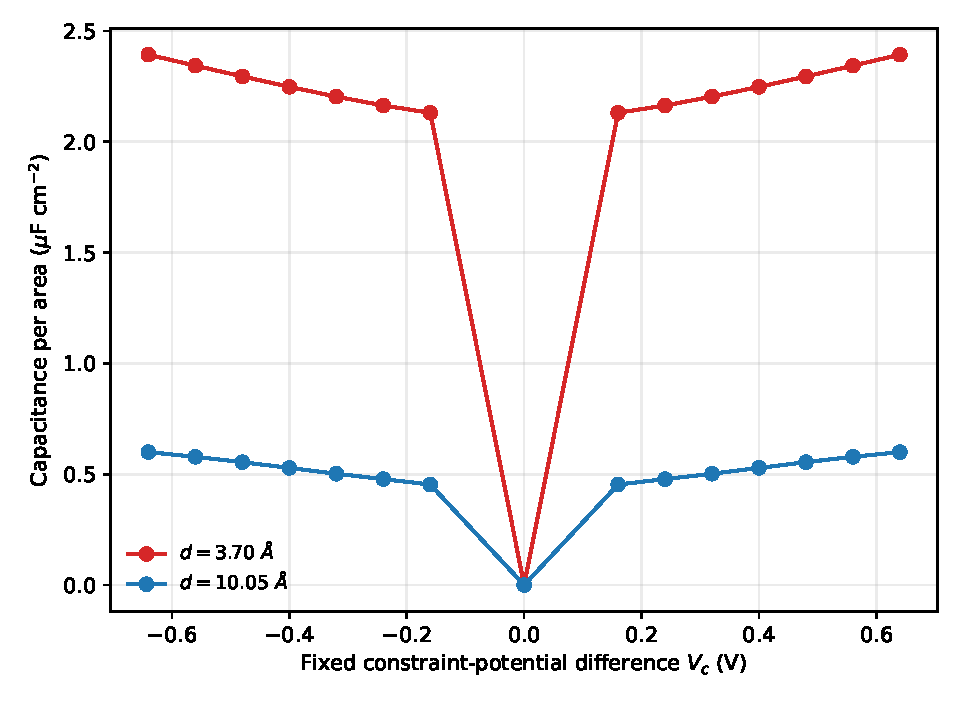
\includegraphics[bb=0 0 461 338,width=0.82\linewidth]{source/paper_reproduction/graphene_two_distance_fig4b_like.pdf}
\caption{Fig.~4(b)-like $C_{\rm total}$. The geometric capacitance is omitted
so that the panel contains only the paper-comparable total quantity.}
\end{figure}
\begin{figure}[htbp]
\centering
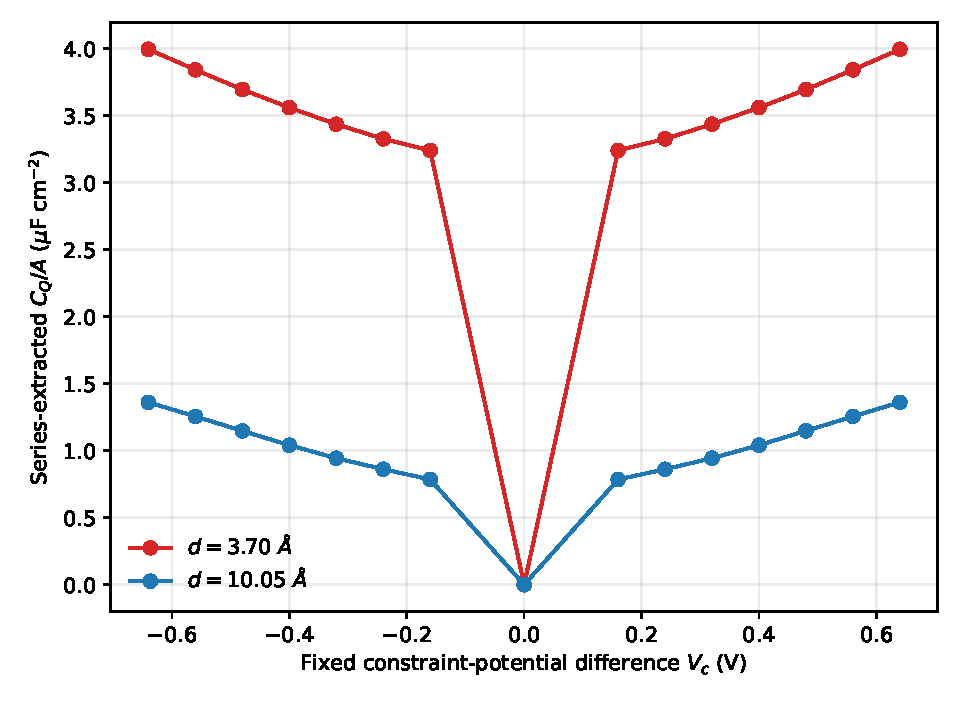
\includegraphics[bb=0 0 461 338,width=0.82\linewidth]{source/paper_reproduction/graphene_two_distance_fig4c_like_cq.pdf}
\caption{Effective $C_Q$ extracted from the series relation.}
\end{figure}

As in the paper, the figures separate $C_{\rm total}$ and $C_Q$. The
A/B-symmetric negative branch and the display origin make each V shape
explicit. $C_{\rm geom}$ is retained in the separate diagnostic file
\texttt{graphene\_two\_distance\_cgeom.pdf}.

The extracted $C_Q$ has a V-like shape resembling Fig.~4(c), but it is not
the same quantity. The paper thermally broadens a high-k-density DOS, whereas
the present value is a residual defined by the series equation. It contains
non-Hartree fixed-potential response and, especially at 3.70~\AA, interlayer hybridization
and charge-partition effects. Its strong distance dependence demonstrates the
distinction. The plotted origin is the paper-style convention; because the
closest computed point is $|V_c|=0.16$~V, the zero-bias value and differential
slope have not been determined.

\section{Small-$V_c$ validation of the Dirac-band response}

The earlier plot assigned zero capacitance at the origin only as a display
convention. We therefore calculated $V_c=0.01$, 0.02, 0.04, 0.06, 0.08,
0.10, 0.12, and 0.16~V for both distances. A $1\times300\times300$ k grid,
chosen as a multiple of three to resolve the K region, a 300~K electronic temperature, and a
$10^{-8}$~Hartree SCF criterion were used. The negative branch follows from
A/B exchange symmetry. The symmetric data were differentiated as
\begin{align}
 \frac{C_{\rm total}^{\rm diff}}{A}&=\frac{e}{A}\frac{dQ}{dV_c},\\
 \frac{C_H^{\rm diff}}{A}&=\frac{e}{A}\frac{dQ}{d\Delta\phi_H},\\
 \frac{1}{C_Q^{\rm diff}}&=\frac{1}{C_{\rm total}^{\rm diff}}
 -\frac{1}{C_H^{\rm diff}}.
\end{align}

\begin{figure}[htbp]
\centering
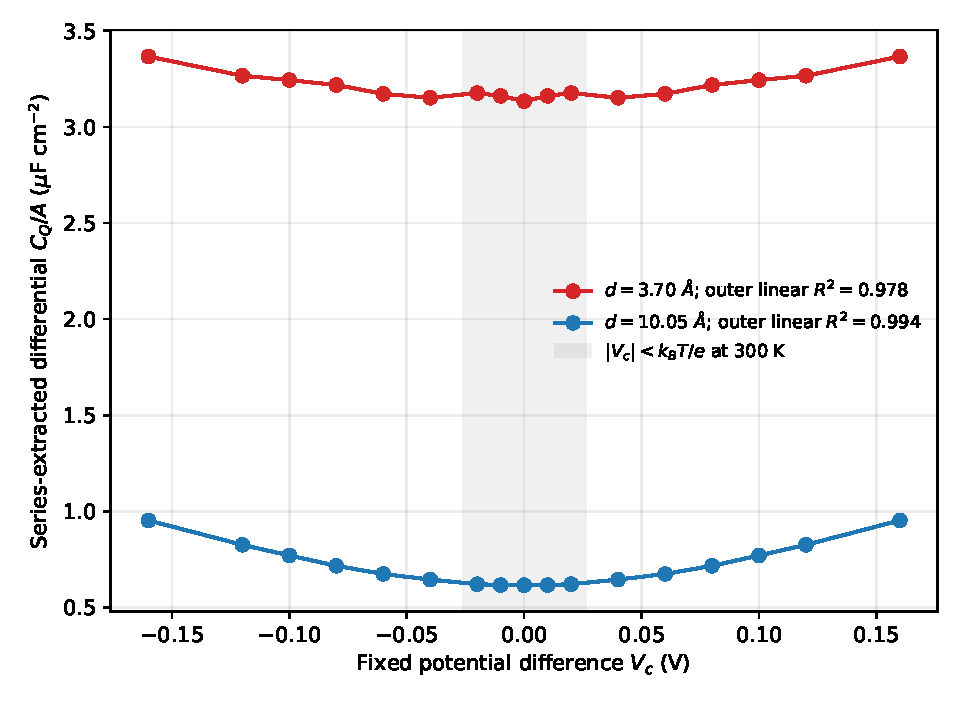
\includegraphics[bb=0 0 461 338,width=0.82\linewidth]{source/paper_reproduction/graphene_dirac_small_vc_cq_diff.pdf}
\caption{Differential effective $C_Q$ from the dense small-$V_c$ sweep. The
shaded interval is $|V_c|<k_BT/e=0.026$~V at 300~K.}
\end{figure}

For $d=10.05$~\AA, $C_Q^{\rm diff}/A$ is
$0.616~\mu$F/cm$^2$ at zero and $0.953~\mu$F/cm$^2$ at 0.16~V. A linear fit
over 0.06--0.16~V gives $R^2=0.994$. The finite rounded minimum on the thermal
scale followed by an almost linear rise with $|V_c|$ is the expected
thermally broadened signature of a graphene Dirac DOS. For $d=3.70$~\AA, the
corresponding values are 3.134 and 3.366, and the response is comparatively
flat; interlayer overlap and hybridization suppress the isolated-Dirac
signature. The fixed-potential series extraction therefore detects the Dirac
character in the weakly coupled system and its loss at short separation,
although it is not a direct DOS integration.

\section{Zero-temperature estimate from the series relation}

The calculation was repeated at an electronic temperature of exactly 0~K,
using ESM on1, the same $1\times300\times300$ k grid and a
$10^{-8}$~Hartree SCF criterion.  The sampled voltages were $V_c=0.005$,
0.01, 0.02, 0.04, 0.06, 0.08, 0.12, and 0.16~V.  No DOS expression is used
in the following estimate.  For each finite-voltage calculation we define the
secant quantities
\begin{align}
 \frac{C_{\rm total}}{A}&=\frac{|Q|e}{A|V_c|}, &
 \frac{C_H}{A}&=\frac{|Q|e}{A|\Delta\phi_H|},\\
 \frac{1}{C_Q}&=\frac{1}{C_{\rm total}}-\frac{1}{C_H}.
\end{align}
Hence the value actually evaluated by the script is
\begin{equation}
 \frac{C_Q}{A}=\frac{|Q|e}
 {A\left(|V_c|-|\Delta\phi_H|\right)}.
\end{equation}
$C_H$ is the effective Hartree electrostatic capacitance, while $C_Q$ is the
effective non-Hartree residual defined by this series decomposition.  These
secant capacitances are distinct from the differential quantities of the
preceding section.

\begin{figure}[htbp]
\centering
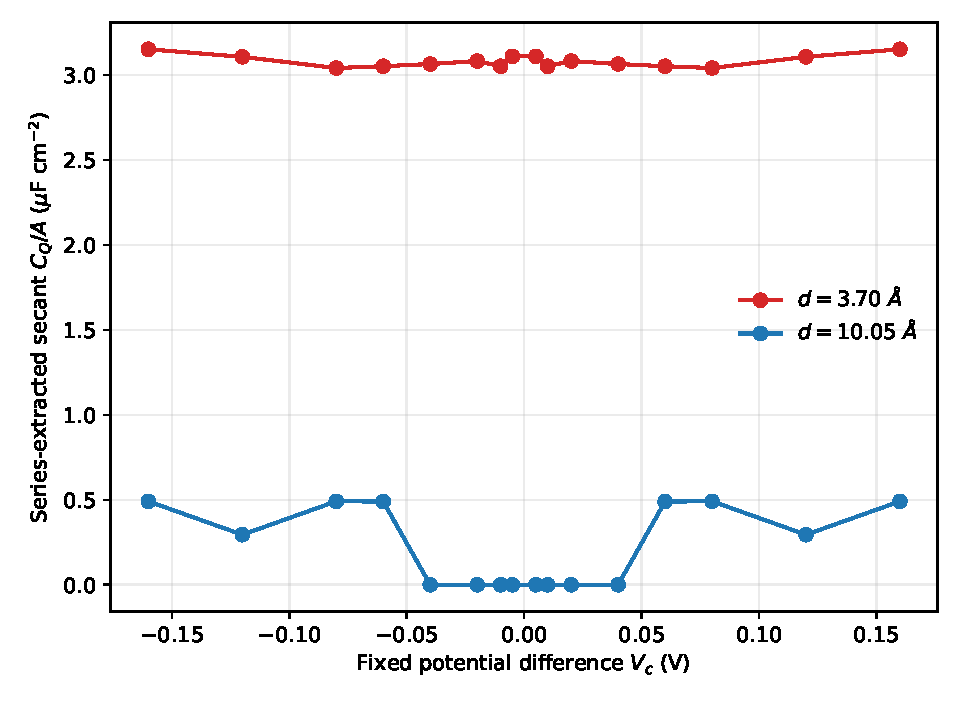
\includegraphics[bb=0 0 461 338,width=0.82\linewidth]{source/paper_reproduction/graphene_dirac_t0_cq_series.pdf}
\caption{Zero-temperature secant $C_Q$ obtained solely from the series
relation.  The negative branch is generated by A/B exchange symmetry.}
\end{figure}

For $d=3.70$~\AA, $C_Q/A$ lies between 3.04 and
$3.15~\mu$F/cm$^2$ and is nearly independent of voltage, as expected when
interlayer overlap and hybridization are strong.  The long-distance results
are
\begin{center}
\begin{tabular}{ccc}
\hline
$V_c$ (V)&$Q$ (e/cell)&$C_Q/A$ ($\mu$F/cm$^2$)\\
\hline
0.005--0.04&0&0\\
0.06&0.00008889&0.490\\
0.08&0.00008889&0.492\\
0.12&0.00008889&0.295\\
0.16&0.00017778&0.491\\
\hline
\end{tabular}
\end{center}
The staircase at $d=10.05$~\AA{} is a finite-k sampling effect rather than a
physical gap.  At exactly zero temperature, occupations on a finite mesh
change only when a discrete sampled state crosses the Fermi level.  Thus the
continuum Dirac limit $C_Q\rightarrow0$ as $V_c\rightarrow0$ appears as a
zero-charge interval followed by discrete steps.  A smooth T=0 V-shaped
differential capacitance requires systematic k-grid convergence; differentiating
the present staircase would not be meaningful.

\section{Validation and limitations}

For a two-layer graphene test with ESM on1 and $d=3.70$~\AA, the
calculation gave $Q=0.00188598$, $|\Delta\phi_H|=0.09225$~V, and
$C/A=6.199~\mu$F/cm$^2$.

The current limitations are:
\begin{enumerate}
 \item no constraint contribution to forces, stress, or total energy;
 \item no persistence of reference populations and $V_c$ in restart files;
 \item basis dependence of Mulliken populations;
 \item no NEGF or multiple independent constraints;
 \item a need to distinguish Hartree, external constraint, and
       electrochemical voltage definitions.
\end{enumerate}

\end{document}
